\documentclass[11pt]{article}

% some definitions for the title page
\newcommand{\reporttitle}{Neural Machine Translation}
\newcommand{\reportdescription}{Attention and stuff}

% load some definitions and default packages
%---------------------------------------------------------------------------
%	PACKAGES AND OTHER DOCUMENT CONFIGURATIONS
%---------------------------------------------------------------------------

\usepackage[twoside]{fancyhdr}
\usepackage{csquotes}

\usepackage[a4paper,hmargin=2.0cm,vmargin=1.0cm,includeheadfoot]{geometry}
% \usepackage{natbib} % for bibliography
\usepackage{biblatex}
\usepackage{tabularx,longtable,multirow,subfigure,caption}%hangcaption
\usepackage{fancyhdr} % page layout
\usepackage{url} % URLs
\usepackage[english]{babel}
\usepackage{graphicx}
\usepackage{rotating}
\usepackage{dsfont}
\usepackage{epstopdf} % automatically replace .eps with .pdf in graphics
% \usepackage{backref} % needed for citations
\usepackage{array}
\usepackage{latexsym}
\usepackage[pdftex,hypertexnames=false,colorlinks]{hyperref} % provide links in pdf (had pagebackref)
\usepackage{booktabs}
\usepackage{wrapfig}
\usepackage{caption}  % Required for \captionof
\usepackage{float} % for H option in figures
\usepackage{amssymb}
\usepackage{amsmath}
\usepackage{amsthm}
\usepackage{mathtools} % for 'dcases*' env.
\usepackage[nottoc]{tocbibind}

%%% Default fonts
\renewcommand*{\rmdefault}{bch}
\renewcommand*{\ttdefault}{cmtt}

%%% Default settings (page layout)
\setlength{\parindent}{0em}  % indentation of paragraph
\setlength{\parskip}{.3em}
\setlength{\itemsep}{0.mm}

\setlength{\headheight}{14.5pt}
\pagestyle{fancy}

\fancyfoot[ER,OL]{\thepage}%Page no. in the left on odd pages and on right on even pages

\fancyfoot[OC,EC]{\sffamily }
\renewcommand{\headrulewidth}{0.1pt}
\renewcommand{\footrulewidth}{0.1pt}
\captionsetup{margin=10pt,font=small,labelfont=bf}

% LISTINGS ammendments
\usepackage{listings}
\usepackage{color}

\definecolor{mygreen}{rgb}{0,0.6,0}
\definecolor{mygray}{rgb}{0.5,0.5,0.5}
\definecolor{mymauve}{rgb}{0.58,0,0.82}

\lstset{ 
  postbreak=\mbox{\textcolor{red}{$\hookrightarrow$}\space},
  backgroundcolor=\color{white},   % choose the background color; you must add \usepackage{color} or \usepackage{xcolor}; should come as last argument
  basicstyle=\footnotesize,        % the size of the fonts that are used for the code
  breakatwhitespace=false,         % sets if automatic breaks should only happen at whitespace
  breaklines=true,                 % sets automatic line breaking
  captionpos=b,                    % sets the caption-position to bottom
  commentstyle=\color{mygreen},    % comment style
%   deletekeywords={...},            % if you want to delete keywords from the given language
%   escapeinside={\%*}{*)},          % if you want to add LaTeX within your code
  extendedchars=true,              % lets you use non-ASCII characters; for 8-bits encodings only, does not work with UTF-8
  firstnumber=1,                % start line enumeration with line 1000
  frame=single,	                   % adds a frame around the code
  keepspaces=true,                 % keeps spaces in text, useful for keeping indentation of code (possibly needs columns=flexible)
  columns=fullflexible,
  keywordstyle=\color{blue},       % keyword style
  language=python,                 % the language of the code
  % morekeywords={*,...},            % if you want to add more keywords to the set
  numbers=left,                    % where to put the line-numbers; possible values are (none, left, right)
  numbersep=5pt,                   % how far the line-numbers are from the code
  numberstyle=\tiny\color{mygray}, % the style that is used for the line-numbers
  rulecolor=\color{black},         % if not set, the frame-color may be changed on line-breaks within not-black text (e.g. comments (green here))
  showspaces=false,                % show spaces everywhere adding particular underscores; it overrides 'showstringspaces'
  showstringspaces=false,          % underline spaces within strings only
  showtabs=false,                  % show tabs within strings adding particular underscores
  stepnumber=1,                    % the step between two line-numbers. If it's 1, each line will be numbered
  stringstyle=\color{mymauve},     % string literal style
  tabsize=2,	                   % sets default tabsize to 2 spaces
  title=\lstname% show the filename of files included with \lstinputlisting; also try caption instead of title
}

% Here, you can define your own macros. Some examples are given below.

\newcommand{\R}[0]{\mathds{R}} % real numbers
\newcommand{\Z}[0]{\mathds{Z}} % integers
\newcommand{\N}[0]{\mathds{N}} % natural numbers
\newcommand{\C}[0]{\mathds{C}} % complex numbers
\renewcommand{\vec}[1]{{\boldsymbol{{#1}}}} % vector
\newcommand{\mat}[1]{{\boldsymbol{{#1}}}} % matrix


\begin{document}

% Include the title page
\begin{titlepage}

    \newcommand{\HRule}{\rule{\linewidth}{0.5mm}} % Defines a new command for the horizontal lines, change thickness here
    
    \center % Center everything on the page
     
    %------------------------------------------------------------------------
    %	HEADING SECTIONS
    %------------------------------------------------------------------------
    
    \textsc{\Large Department of Computing}\\[0.5cm] 
    \textsc{\large Imperial College of Science, Technology and Medicine}\\[0.5cm] 
    
    %------------------------------------------------------------------------
    %	TITLE SECTION
    %------------------------------------------------------------------------
    
    \HRule \\[0.4cm]
    { \huge \bfseries \reporttitle}\\ % Title of your document
    \HRule \\[0.4cm]

    \textit{\reportdescription}
    
    \vspace{2em}

    %------------------------------------------------------------------------
    %	AUTHOR SECTION
    %------------------------------------------------------------------------
    
    \large \emph{Author: Anton Zhitomirskiy}

    \vspace{1em}

    \global\let\newpagegood\newpage
    \global\let\newpage\relax
    
\end{titlepage}

\global\let\newpage\newpagegood

\tableofcontents

\clearpage

\section{Machine Translation}

At the highest level, given a document in source language, produce a translation in a target language. This motivates the encoder decoder models that we've seen.

\section{Statistical Machine Translation}

It is a pipeline of the models: Alignment model, Translation model, and Lanugage model.

Uses parallel corpa as its training set. A prallel corpa is that we have aligned sentences: i.e. an english sentence and its corresponding french sentence.

\begin{figure}[H]
    \centering
    \includegraphics*[width=.6\linewidth]{figures/smt-idea.png}
\end{figure}

\begin{itemize}
    \item \textbf{Parallel dataset} - paired sentences between two different languages (we want to construct correlations between the phrase that happens in one language and translation into another.)
    \item \textbf{Alignment model} - responsible for extracting the phrase pairs    
    \item \textbf{Translation model} - Contains phrases alongside their translation. A lookup table, what is the porbability of the word `go' appearing in the contex of this target. statistics over large pairs of parallel texts can
    help identify parallel phrases
    \item \textbf{Corpus} of target monolongual corpus - this is used to get n-grams from the data (what is the probability of this n-gram given this data?)
    \item \textbf{Language model} - contains the probability of target language phrases 
\end{itemize}

\subsection{How to perform translations}

\begin{itemize}
    \item The objective is to find $p(t|s)$; given a source sentence, s, we want target sentence, t. Language models can be trained on monolingual data\footnote{``It contains texts in one language only'' \href{https://www.sketchengine.eu/corpora-and-languages/corpus-types/}{here}} that gives us probability of a phrase occurring in that language.
    \item The translation model is the ``objective'' flipped. How likely is the source phrase going to occur given a cnadidate translation t. We will have multiple candidate translations. 
    \item These probabilities/likelihoods are built from statistics of our bilingual parallel corpus.
    \item With this information we can apply Bayes rule to obtain $p(t|s)$.
    \begin{equation*}
        p(t|s) = \frac{p(t)p(s|t)}{p(s)}
    \end{equation*}
    \item p(s) is just a normalising factor. It doesn't contain t so is irrelevant to     obtaining what we're interested in: the actual model
    \item The actual model is the argmax. Here - pick the phrase that has the highest
    probability of the product of the 2 terms $p(t)$ (language model) and $p(s|t)$
    (translation model)
\end{itemize}

\subsection{Example}

\begin{figure}[H]
    \centering
    \includegraphics*[width=.9\linewidth]{figures/example-translation-1.png}
\end{figure}

The first part is to use the translation model, so given these target phrases which have been built by the alignment model and the probabilities which are in the translation modle, what is the most likely candidate, the most likely translation candidate for this given source sentence. 

The second part is the lnaguage model itself, which will take each one of these candidates and compute how likley they are to actually appear in target data.

\subsection{Downsides}

\begin{itemize}
    \item \textbf{Sentence Alignment}
    
    In parallel corpora single sentences in one language can be translated into
    several sentences in the other and vice versa. Long sentences may be
    broken up, short sentences may be merged. There are even some
    languages that use writing systems without clear indication of a sentence
    end (for example, Thai).

    \item \textbf{Word Alignment}
    
    Is about finding out which words align in a source-target sentence pair

    One of the problems presented is function words that have no clear
    equivalent in the target language. For example, when translating from
    English to German the sentence "John does not live here," the word
    "does" doesn't have a clear alignment in the translated sentence "John
    wohnt hier nicht."

    \item \textbf{Statistical anomalies}
    
    Real-world training sets may override translations of, say, proper nouns.
    An example would be that "I took the train to Berlin" gets mis-translated as
    "I took the train to Paris" due to an abundance of "train to Paris" in the
    training set.

    \item \textbf{Idioms}
    
    Only in specific contexts do we want idioms to be translated. For example,
    using in some bilingual corpus (in the domain of Parliment), "hear" may
    almost invariably be translated to "Bravo!" since in Parliament "Hear,
    Hear!" becomes "Bravo!”

    \item \textbf{Out of vocabulary words}
\end{itemize}

\section{Neural Machine Translation}

\begin{figure}[H]
    \centering
    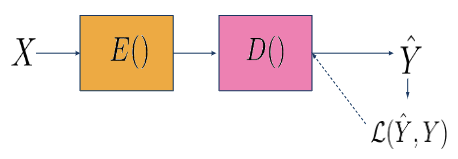
\includegraphics[width=.5\linewidth]{figures/encoder-decoder.png}
\end{figure}

\begin{itemize}
    \item Encoder function $E()$ - Represents the source as a latent encoding we cannot interpret
    \item Decoder function $D()$ - Generates a target from the latent encoding.
    \item Input sequence (source) $X=\{x_1,\dots, x_i\}$
    \item Output sequence (target) $Y=\{y_1,\dots, y_i\}$
    \item Loss over out outputs; our predicted output given our real output.
\end{itemize}

\subsection{RNNs}

\begin{figure}[H]
    \centering
    \subfigure[vanilla RNN. The hidden state represents the whole sequence]{\includegraphics*[trim={3px 0 0 0}, clip, width=.8\linewidth]{figures/RNN.png}}
    \subfigure[bidirectional RNN]{\includegraphics*[width=.8\linewidth]{figures/RNN-bidirectional.png}}
\end{figure}

Using a BiRNN is appropriate for encoding the source as we’re not trying to
predict the source. We have access to the whole thing at inference time. Using
a BiRNN, and reading information from both sides, allows us to gain a more
information dense representation of our sequence

We can get a hint of representation for each word and hit a representation for each word. The inner representation of each word consists of the forward direction concatentated witht he backwards direction for that particular word or particular token concatenated together.

\subsection{Naiive implementataion of machine translation}

\begin{figure}[H]
    \centering
    \includegraphics*[width=\linewidth]{figures/naiive-rnn.png}
\end{figure}

Given an input seqeunce we want to generate the output sequence. We get a c, the context vector, which we initialize our language model (the pink model, the decoder) which we initialize with the hidden state. The context comes from the encoder.

In the bidirectional RNN case, there are two ways that we can compute the context vector. 

\begin{enumerate}
    \item Simply take the lsat representations form the forward and backward direction and calculate them together
    \item Average across each one of those representations adn theat can form our context vector (there is a leakage here)
\end{enumerate}

The dimension of $C$ if dimensionality of the model is $d$, then we either have to set s in $R^{2d}$ or project $c$ down to $R^d$.

\subsection{Teacher Forcing}

\begin{figure}[H]
    \centering
    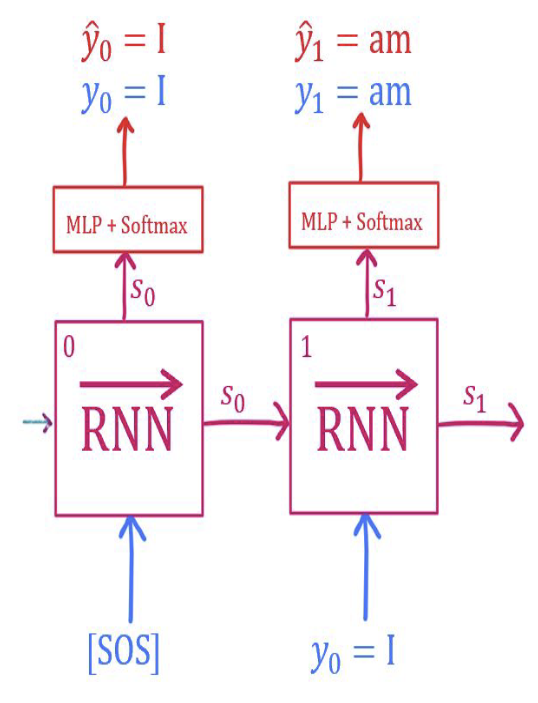
\includegraphics[width=.3\linewidth]{figures/teacher-forcing.png}
\end{figure}

Decoder is auto-regressive only during inference

During training, we use teacher forcing. We are feeding the ground truth token ot the enxt deconder cell: $S_t$ makes a prediciton, we calculate loss $\mathcal L (\hat y_t, y_t)$ then feed $y_t$ to decoder cell at $t+1$.

We use teacher forcing with a \textbf{ratio}. I.e. we well teacher force
ratio\% of time. The ratio can be 100\% (i.e. full teacher forcing), 50\%, or you
can even anneal it during training

If at timestamp $t$ the model makes a wrong prediction $\hat y_t$ with standard autoregressive modelling, if we fed this back inot decoder at call $t+1$ our model has (potentially) incorrect context. It will use this incorrect context to decode $\hat y_{t+1}$; we will likley produce another incorrect word. This leads to an accumulation of errors, which is difficult to optimze over.

Teacher forcing creates a phenomenon called \textbf{Exposure Bias}.

Exposure Bias is when the data distributions the model is conditioned on vary between training and inference. In this case, if we set teacher forcing to 100\%, then the model is never conditioned on its own predictions. So during inference, when the model uses the previously generated words as context, it is different than what it has seen in training.

\subsection{Implementation}

\begin{enumerate}
    \item Minimse negative log likelihood loss: \begin{equation}
        -\sum^T_{t=1}\log p(\hat y_t | y_{<t}, c)
    \end{equation}
    Here, we assume that we have a teacher forcing ratio of 100\%.
    Also, $y_{<t}$ means all the tokens up to the $t$'th time step. With teacher ratio of less than 100\%, this would be written as a joint of the previosuly decoded tokens (whether they're sampled or the ground truth).
    \item c is the context vector output by the encoder \begin{equation}
        c = E(X)
    \end{equation}
    \item $\hat y_t$ is the decoder output: \begin{equation}
        \hat y_t = \sigma(W_o \cdot D(y_{<t}; c)), \quad W_o \in \mathbb R^{d\times o}
    \end{equation}
    Here, $o$ is the output covabulary size. Sigma, is an activation funciton SOFTMAX becuase we're classifying over multiple things.
    \item Encoder and decoder are connected... so perform BPTT as normal.
\end{enumerate}

\subsubsection{Why is this suboptimal}

\begin{itemize}
    \item We're tying to encode a long sequence in a fixed dimensional representation. For longer sequence lengths, the ability to retain all the source information in this vector diminishes.
    \item From the decoder side of things, as more words get decoded and the hidden state gets updated to incorporate the previously generated words, information from the context vector may start to diminish.. This is related to:
    \item vanishing gradients and the lack of ability to `remember' things from earlier parts of the sequence
\end{itemize}

\subsubsection{Fixes}

\begin{itemize}
    \item $c$ is the entire context for the decoder, wheras the encoder can give us access ot more infromatino that just $c$ (since we're using bidirectional encodings for each word, we know the context from both ends of the sentence) Thus if we could utilise these more fine-grained encodings, we wouldn't suffer from the loss of information that we get from a context vector.
    \item We may find out which source words are most important to look at for our current timestep of decoding.
    \item What if, during decoding, the current decoding timestep could look at all the source words, and fin dout which source words are most improtant to its current stage of decoding? Then we could `pay attention' to those words more than the other words?
\end{itemize}

\section{Attention}

Attention enables weighting individual tokens in the input w.r.t something else. It allows us to look at individual tokens in the input and decide how much weighting a token should have with respect to the current timestep of decoding. The weighting does ont necessarily need ot be in respect to decoding.

\subsection{Process}

\begin{enumerate}
    \item For every decoding timestamp we have, we now have a context vector for that decoding time step.
    \item We have $i$ hidden states, which are all the encoder's hidden states. We loop over them and multiply it by some $\alpha$ value which is a scalar between 0 and 1.
    
    \begin{equation}
        c_t = \sum^I_{i=1}\alpha_ih_i
    \end{equation}

    \item We try to decode the $y_t$'th word and we have access all bi-directional states at every decoding timestep.
    \item Before we decode $y_t$ we're going to feed all our encoder hidden states AND the decoder hidden state $s_{t-1}$ to our attention module. 
    \item The module will output a context vector, $c_t$.
    \item $c_t$ is a dynamic and contextualised representation. It uses the decoder hidden state information to try and figure out which source words are most important when for decododing $y_t$. 
    \item We send $c_t$ to the $t$'th RNN step, alongside the previously generated token $y_{t-1}$. 
    \item One final change that the methodology introduced (not strictly related to attention itself), is that the output projection layer now laso takes in $c_t$ and the word embeddings for $y_{t-1}$ alongside $s_t$ to predict the $t$'th word.
    \item Within $c_t$ the $\alpha_i h_i$ multiplication is a key point of attention. It applies a ``mask'' to each of our hidden states. Low energy values tend to 0 which measn that we do not need that words infromatino to decode the next word
    \item Here, the alignment funciton is essentially a 2 layered MLP. The first layer combines the decoder hidden state with all our encoder hidden states, the second layer (v) uses this contextulaised representaiton to predict an energy score: i.e. unnormalised ``importance'' of each of teh source words.
\end{enumerate}

\begin{figure}[H]
    \centering
    \fbox{\includegraphics[page=29, trim=5.2cm 14cm 4.5cm 2.1cm, clip, width=.89\linewidth]{Lecture 4 - Machine Translation.pptx (with notes).pdf}}
\end{figure}

\subsubsection{Example}

\begin{figure}[H]
    \centering
    \subfigure[These are our bidirectionally encoded encoder hidden states where for each word we have some $d$ dimensional representation of the word]{
        \fbox{\includegraphics[page=30, trim=3.2cm 14cm 3.2cm 2.1cm, clip, width=.45\linewidth]{Lecture 4 - Machine Translation.pptx (with notes).pdf}}
    }
    \subfigure[We have $I$ words, and each word is encoded in $2D$ dimensions. Where $D$ is the model dimensionality. It is 2D because we have forward and backwards representations.   We project the last hidden state to obtain a $D$ dimensional vector]{
        \fbox{\includegraphics[page=31, trim=3.2cm 14cm 3.2cm 2.1cm, clip, width=.45\linewidth]{Lecture 4 - Machine Translation.pptx (with notes).pdf}}
    }
\end{figure}

\begin{figure}[H]
    \centering
    \subfigure[To feed $C$ into our decoder, we double the dimensionality that is in our encoder o or have a projection layer to reduce the dimensionality into $d$ dimensions. Then the decoding process can begin. The decoder RNN has inputs INIT vector (the projected version of the output of the encoder), and the SOS token (start of sequence).]{
        \fbox{\includegraphics[page=32, trim=3.2cm 14cm 3.2cm 2.1cm, clip, width=.45\linewidth]{Lecture 4 - Machine Translation.pptx (with notes).pdf}}
    }
    \subfigure[Before we generate the next prediced word, we run the attention mechanis. The attention mechanism takes ALL the encoder hidden states as input, and teh decoder hidden state being inputted to the RNN to decode the current word. The attention is performed over these inputs, and the module outputs a context vector specific to this decoding time step. ]{
        \fbox{\includegraphics[page=35, trim=3.2cm 14cm 3.2cm 2.1cm, clip, width=.45\linewidth]{Lecture 4 - Machine Translation.pptx (with notes).pdf}}
    }
    \subfigure[It gives us 2 outputs: our decoder hidden state vector ($s_0$), and the prediction first word]{
        \fbox{\includegraphics[page=36, trim=3.2cm 14cm 3.2cm 2.1cm, clip, width=.45\linewidth]{Lecture 4 - Machine Translation.pptx (with notes).pdf}}
    }
    \subfigure[We then start decoding the next word, if using teacher forcing, we feed the ground truth word as input]{
        \fbox{\includegraphics[page=37, trim=3.2cm 14cm 3.2cm 2.1cm, clip, width=.45\linewidth]{Lecture 4 - Machine Translation.pptx (with notes).pdf}}
    }
    \subfigure[Again, we run the attention process. We take in ALL encoder hidden states as
    input, and the previously outputted decoder hidden state]{
        \fbox{\includegraphics[page=38, trim=3.2cm 14cm 3.2cm 2.1cm, clip, width=.45\linewidth]{Lecture 4 - Machine Translation.pptx (with notes).pdf}}
    }
    \subfigure[Attention is going to give us $\alpha$ values for EACH encoded word. These will be between 0 and 1. We're going to scale each encoded word by $\alpha$ and sum them all together to obtain a context vector.]{
        \fbox{\includegraphics[page=39, trim=3.2cm 14cm 3.2cm 2.1cm, clip, width=.45\linewidth]{Lecture 4 - Machine Translation.pptx (with notes).pdf}}
    }
\end{figure}

\subsection{How to obtain energy scores?}

\emph{For every source word}, $i$, we're going to obtain a value:

\begin{equation}
    \underbrace{e_i}_{\ref{eq:ei}} = \underbrace{a}_{\ref{eq:a}}(\underbrace{s_{t-1}}_{\ref{eq:st-1}}, \underbrace{h_i}_{\ref{eq:hi}}) = \underbrace{v^T}_{\ref{eq:vT}} \overbrace{\tanh}^{\ref{eq:tanh}}(\underbrace{W}_{\ref{eq:W}}s_{t-1} \overbrace{+}^{\ref{eq:+}} \underbrace{U}_{\ref{eq:U}} h_i)
\end{equation}

\begin{enumerate}
    \item \label{eq:ei} $e_i \in \mathbb R ^1$. The unnormalized energy source for each source word $i$. ``How important is this word to the current decoding step?''
    \item \label{eq:a} A learnt neural network 
    \item \label{eq:st-1} $s_{t-1} \in \mathbb R ^{D\times 1}$  Previous decoder hidden state 
    \item \label{eq:hi} $h_i \in \mathbb{R}^{2D\times 1}$ Encoder hidden state for the $i$'th word.
    \item \label{eq:vT} $v^T \in \mathbb R^{D\times 1} \wedge v \in \mathbb R^{1\times D}$. $v$ is responsible for creating the energy score.
    \item \label{eq:W} $W \in \mathbb R^{D\times D}$. similarly to $U$, we project $s_{t-1}$ via $W$ which also results in a $D$-dimensional vector
    \item \label{eq:U} $U \in \mathbb R^{D\times 2D}$. We project/transform $h_i$ to a D-dimensional vector via a learned weights matrix $U$.
    \item \label{eq:+} The plus is important here because it mixes the infromation from the decoder and the hidden states together
    \item  \label{eq:tanh} Here, $\tanh$ is just a non-linearity we're applying to it. We could have used another activation function if we wanted to.
\end{enumerate}

The energy scores then get normalised.

\begin{figure}[H]
    \centering
    \fbox{\includegraphics[page=55, trim=3.2cm 14cm 3.2cm 2.1cm, clip, width=.7\linewidth]{Lecture 4 - Machine Translation.pptx (with notes).pdf}}
    \caption*{We now have all our energy scores, but they are currently unnormalised. We normalize them by sending all the enrgy scores to a softmax function. This gives us $\alpha$ values between 0 and 1. Therefore, they all sum to 1.}
\end{figure}

\subsubsection{Example continued}

\begin{figure}[H]
    \centering
    \subfigure[Add all together to obtain $c_t$ - our context vector]{
        \fbox{\includegraphics[page=59, trim=3.2cm 14cm 3.2cm 2.1cm, clip, width=.45\linewidth]{Lecture 4 - Machine Translation.pptx (with notes).pdf}}
    }
    \subfigure[Continuing from where we were in our diagram, we then output the context vector for the $t=1$ word (c1). This forms our 3rd input to the current RNN step (alongside $s_0$ and an input word)]{
        \fbox{\includegraphics[page=60, trim=3.2cm 14cm 3.2cm 2.1cm, clip, width=.45\linewidth]{Lecture 4 - Machine Translation.pptx (with notes).pdf}}
    }
    \subfigure[The RNN uses these 3 inputs to output decoder hidden state $s_t$ and a prediction (am)]{
        \fbox{\includegraphics[page=61, trim=3.2cm 14cm 3.2cm 2.1cm, clip, width=.45\linewidth]{Lecture 4 - Machine Translation.pptx (with notes).pdf}}
    }
    \subfigure[Repeat the process until we hit our max length]{
        \fbox{\includegraphics[page=62, trim=3.2cm 14cm 3.2cm 2.1cm, clip, width=.45\linewidth]{Lecture 4 - Machine Translation.pptx (with notes).pdf}}
    }
\end{figure}

\subsection{Visualising the attention}

\begin{minipage}[l]{.6\linewidth}
    \centering
    \fbox{\includegraphics[page=64, trim=3.2cm 14cm 3.2cm 2.1cm, clip, width=\linewidth]{Lecture 4 - Machine Translation.pptx (with notes).pdf}}
\end{minipage}\hfill
\begin{minipage}[r]{.35\linewidth}
    We can visualise our attention values to see which source words were looked at most when decoding a target word - I.e. when we're decoding the word person, in German, we're looking strongly at ``person'' in English, and also ``the''.
\end{minipage}

\subsection{Conclusion}

\begin{minipage}[l]{.6\linewidth}
    \centering
    \fbox{\includegraphics[page=65, trim=3.2cm 14cm 3.2cm 2.1cm, clip, width=\linewidth]{Lecture 4 - Machine Translation.pptx (with notes).pdf}}
\end{minipage}\hfill
\begin{minipage}[r]{.35\linewidth}
    We see that longer sentences are better handled with attention. We have dynamic represetntaion for each time tsep that we're decoding.
\end{minipage}

\section{Evlauation metrics of MT/NLG systems}

\begin{itemize}
    \item Human evaluation (best but expensive)
    \item Automatic evaluation: proxies to gaugae how effective the machine generated output is \begin{itemize}
        \item Fast/proxy mesaures for evaluation
        \item Often based on count statistics of n-grams
    \end{itemize}
\end{itemize}

\subsection{BLEU}

BLEU reports a modified precision metric for each level of n-gram. Credit is assigned as the maximum amount of time each unique n-gram appears over all the references. Multiple references are recommended (not a strict requirement).

\begin{minipage}[l]{0.5\linewidth}
    \centering
    \fbox{\includegraphics[page=69, trim=3.2cm 14cm 3.2cm 2.1cm, clip, width=.9\linewidth]{Lecture 4 - Machine Translation.pptx (with notes).pdf}}
\end{minipage}\hfill
\begin{minipage}[l]{0.5\linewidth}
    First calculate the number of unique n-grams in our Hypothesis. ModifiedPrecision-1 means uni-grams. Then we look at the n-gram overlap bewteen the unique ngrams in our Hypothesis and all n-grams in our References. We work out the number of unique overlaps beteween the unique ngrams and all the Refs (there are two instances of the in the first reference, and 1 in the second). Then we obtain our modified-precision scores: the total unique overlap divided by the number of n-grams in our Hyp.
\end{minipage}

\subsubsection{Modified Precision Score}

\begin{equation}
    \text{Modified Precision score } p_n = \frac{\text{Total Unique Overlap}_n}{\text{Total n-grams}}
\end{equation}

Here, we have an example sentence in french ``Le chat est sur le table'' with references (shown on the example) and two outputs, \texttt{MT\_Bad} and \texttt{MT\_Ok}.

\begin{figure}[H]
    \centering
    \subfigure[MP-1: Question, answer below:]{
        \fbox{\includegraphics[page=70, trim=3.2cm 16.5cm 3.2cm 3.5cm, clip, width=.45\linewidth]{Lecture 4 - Machine Translation.pptx (with notes).pdf}}
    }
    \subfigure[MP-2: Question, answer below:]{
        \fbox{\includegraphics[page=71, trim=3.2cm 16.5cm 3.2cm 3.5cm, clip, width=.45\linewidth]{Lecture 4 - Machine Translation.pptx (with notes).pdf}}
    }
    \subfigure[``What are the unique n-grams that exist (in the \texttt{MT\_OK})? We have `the', `cat', `on', `mat'. Then we work out the maximum number of times that there is an overlap betwen each one of our unique n-grams and we see: `the', `cat', `on', `the' (we see `the' twice in our references) and `mat'. Then, the total number of machine translated n-grams is 7 so the modified precision socre is 5'']{
        \fbox{\includegraphics[page=72, trim=3.2cm 16cm 3.2cm 3.5cm, clip, width=.45\linewidth]{Lecture 4 - Machine Translation.pptx (with notes).pdf}}
    }
    \subfigure[\texttt{total\_unique\_overlap} measures the \textbf{UNIQUE} occurrences, not only the intersection between the two reference sentences. Here, underlined in bold black are the unique occurrences from the unique\_ngrams list. We do not include the end of sentence reference here because we are testing the produced output. EOS is somethind done within the model representation. \texttt{total\_ngrams} is not unique, there are 6 in the \texttt{MT\_OK}.]{
        \fbox{\includegraphics[page=73, trim=3.2cm 16cm 3.2cm 3.5cm, clip, width=.45\linewidth]{Lecture 4 - Machine Translation.pptx (with notes).pdf}}
    }
    \caption{Further discussion seems to point that the \texttt{total\_unique\_overlap} is taking the max of occurences of each of the n-grams that appear at the sentence level. So in the 1-gram model, we have 2 `the' in reference 1, and 1 `the' in reference 2. So the max is 2.}
\end{figure}

\subsubsection{BLEU score}

Measures precision of n-gram matches (typically up to 4-grams). Scaled by a Brevity Penalty (BP), it is used to mostly encourage the hypothesis to be of a simlar length to the reference.

\begin{equation}
    \texttt{BLEU-4} = \texttt{BP}(\prod^4_n p_n)^\frac{1}{4}, \quad \texttt{BP} = \min(1, \frac{\text{MT Output Length}}{\text{Reference Length}})
\end{equation}

\subsubsection{Downside}

A shortcoming of BLEU is that it focuses a lot on the precision between Hyp and Ref, but not the recall.

\subsection{Chr-F \& TER}

\subsubsection{Chr-F}

Chr-F is a character n-gram $F_\beta$ score. 

\begin{itemize}
    \item Balances \textbf{character precision} \begin{itemize}
        \item percentage of n-grams in the hypothesis which have a acounterpart in the reference
    \end{itemize}
    \item and \textbf{character recall} \begin{itemize}
        \item percentage of character n-grams in the reference which are also present in the hypothesis.
    \end{itemize}
\end{itemize}

\subsubsection{TER: Translation Error Rate}

Minimum \# of edits required to change a hypothesis into one of the references. TER is performed at the word level, and the ``edits'' can be a: Shift, Insertion, Substitution and Deletion. TER balances these edits to build a metric

\subsection{ROUGE}

\begin{minipage}[l]{.5\linewidth}
    \centering
    \fbox{\includegraphics[page=79, trim=3.2cm 14cm 3.2cm 2.1cm, clip, width=.9\linewidth]{Lecture 4 - Machine Translation.pptx (with notes).pdf}}
\end{minipage}\hfill
\begin{minipage}[r]{.5\linewidth}
    \begin{itemize}
        \item ROUGE balances both precision and recall via the F-Score.
        \item Though originally a translation metric, ROUGE is more common in captioning/summarization literature than translation. Obviously it can be used for translation though.
        \item ROUGE-n measures the F-score of n-gram split references and system outputs  
        \item ROUGE-L is the F-score of the LCS between the references and system outputs. The subsequence does not have to be consecutive
        \item For example… given this Ref and Hyp: 
        \item Other variants of ROUGE such as ROUGE-S, ROUGE-W which incorporate skip grams and/or weighting
    \end{itemize}
\end{minipage}

\subsection{METEOR}

\begin{minipage}[l]{.5\linewidth}
    \centering
    \fbox{\includegraphics[page=82, trim=3.2cm 14cm 3.2cm 2.1cm, clip, width=.9\linewidth]{Lecture 4 - Machine Translation.pptx (with notes).pdf}}
\end{minipage}\hfill
\begin{minipage}[r]{.5\linewidth}
    \begin{itemize}
        \item METEOR is more modern and a better metric than BLEU, though for some reason the NMT community still adopts BLEU a lot more frequently. You will find METEOR in other generation tasks such as summarization and captioning
    \end{itemize}
\end{minipage}

\subsection{N-gram methods have shortcomings}

\begin{minipage}[l]{.5\linewidth}
    \centering
    \fbox{\includegraphics[page=83, trim=3.2cm 14cm 3.2cm 2.1cm, clip, width=.9\linewidth]{Lecture 4 - Machine Translation.pptx (with notes).pdf}}
\end{minipage}\hfill
\begin{minipage}[r]{.5\linewidth}
    \begin{itemize}
        \item To humans, system A makes more sense, as it catches more meaning behind the meaning of the reference
        \item This n-gram based method cannot capture the context behind sentences.
        \item Other metrics might be slightly more robust than this, but fundamentally n-gram methods cannot take into account valid candidates/machine outputs which may use synonyms instead of a word in the reference.
    \end{itemize}
\end{minipage}

\subsection{BertScore}

Not count based. Bert is a trained language model that can give oyu contextual representations of tokens/words. It's not used so much for translation, but still a good metric for most sequence-to-sequence tasks. The biggest drawback is now not the n-gram matching, rather, the scores can vary if evaluated against different BERT models.

\begin{figure}[H]
    \centering
    \fbox{\includegraphics[page=84, trim=3.2cm 14cm 3.2cm 2.1cm, clip, width=.9\linewidth]{Lecture 4 - Machine Translation.pptx (with notes).pdf}}
    \caption*{Performs a pairwise cosine similarity between each word in the reference and each word in the candidate.}
\end{figure}

If you have a sequence to sequence task then bert score is the metric you should be using. So if you have summarization, audio transcription, generative question answering then BERT score is a good score to use.

\section{Inference}

During training, we used teacher forcing. Now we don't have access to the ground truth. During inference we can either perform:

\subsection{Greedy decoding}

Outputs the most likely word at each time step (i.e. an argmax). It is fast, but doesn't look into the future. But as we decode the rest of the sentence, it might be worse than we thought. If we were able to see what the future candidates might be, we might be able to predict a better word for the current time step.

\begin{figure}[H]
    \centering
    \fbox{\includegraphics[page=87, trim=6cm 14.5cm 6cm 5.8cm, clip, width=.6\linewidth]{Lecture 4 - Machine Translation.pptx (with notes).pdf}}
\end{figure}

\subsection{Beam search}

Instead of choosing the best token to generate at each time-step we keep $k$ possible tokens at each step. In practice, $k$ is normally between 5-10. Note that we will end up with $k$ hypothesis at the end of decoding. Decoding finishes when we hit an EOS token. For example, here is $k=2$.

\begin{figure}[H]
    \centering
    \subfigure[$t=0$ `arrived' and `the' are the 2 most likley words]{
        \fbox{\includegraphics[page=88, trim=6cm 14.3cm 6cm 4.9cm, clip, width=.3\linewidth]{Lecture 4 - Machine Translation.pptx (with notes).pdf}}
    }
    \subfigure[$t=1$ for each word, decode the next k. We end up with the green nodes. Then, prune all but the top-k]{
        \fbox{\includegraphics[page=89, trim=6cm 14.3cm 6cm 4.9cm, clip, width=.3\linewidth]{Lecture 4 - Machine Translation.pptx (with notes).pdf}}
    }
    \subfigure[$t=2$ repeat. Now we have the next green, and lets predict 2 times steps into the future and keep track of the 2 tokens that give the highest likelihood for those time steps.]{
        \fbox{\includegraphics[page=90, trim=6cm 14.3cm 6cm 4.9cm, clip, width=.3\linewidth]{Lecture 4 - Machine Translation.pptx (with notes).pdf}}
    }
\end{figure}

\begin{figure}[H]
    \centering
    \vstretch{.8}{
            \fbox{\includegraphics[page=91, trim=3.2cm 14cm 3.2cm 2.1cm, clip, width=.95\linewidth]{Lecture 4 - Machine Translation.pptx (with notes).pdf}}
        }
\end{figure}

\subsection{Temperature sampling}

Introduces stochasticity into the decoder step. This is a problem with the two above; they are deterministic. 

\begin{figure}[H]
    \centering
    \vstretch{.8}{
            \fbox{\includegraphics[page=92, trim=3.2cm 14cm 3.2cm 2.1cm, clip, width=.95\linewidth]{Lecture 4 - Machine Translation.pptx (with notes).pdf}}
        }
\end{figure}

\section{Tricks | how to improve performance of models}

\subsection{Data Augmentation}

\subsubsection{Backtranslation}

Lets translate the source into one language and translate it back. The hope is, that once translated back the semantics is the same but syntactically it may be different.

\begin{itemize}
    \item Train/use a separate target $\rightarrow$ source model
    \item Translate target monolingual corpora to source using the model
    \item Train the actual source $\rightarrow$ target model with the additional data
    \item Ideally changes the syntax of source while keeping the same semantics. Downsides: adds noise to the source
\end{itemize}


\subsubsection{Synonym replacement}

\begin{itemize}
    \item Use dictionary \& syntax trees to find appropriate synonyms
    \item Use word embeddings \& nearest neighbours to find synonyms.
\end{itemize}

\subsubsection{Batching, PAdding and Sequence Length}

\begin{itemize}
    \item Group similar length sentences together in the batch
    \item train your model on simpler/smaller sequence lengths first.
\end{itemize}

\end{document}
